\chapter{Multiple and logistic regression}
\label{multipleRegressionAndANOVA}
\label{multipleAndLogisticRegression}

The principles of simple linear regression lay the foundation for more sophisticated regression methods used in a wide range of challenging settings. In Chapter~\ref{multipleAndLogisticRegression}, we explore multiple regression, which introduces the possibility of more than one predictor, and logistic regression, a technique for predicting categorical outcomes with two possible categories.




\section[Introduction to multiple regression]{Introduction to multiple regression \sectionvideohref{youtube-sQpAuyfEYZg&list=PLkIselvEzpM5f1HYzIjFt52SD4izsJ2_I}}
\label{introductionToMultipleRegression}

\index{multiple regression|(}

Multiple regression extends simple two-variable regression to the case that still has one response but many predictors (denoted $x_1$, $x_2$, $x_3$, ...). The method is motivated by scenarios where many variables may be simultaneously connected to an output.

\index{data!mario\_kart|(}

We will consider Ebay auctions of a video game called \emph{Mario Kart} for the Nintendo Wii. The outcome variable of interest is the total price of an auction, which is the highest bid plus the shipping cost. We will try to determine how total price is related to each characteristic in an auction while simultaneously controlling for other variables. For instance, all other characteristics held constant, are longer auctions associated with higher or lower prices? And, on average, how much more do buyers tend to pay for additional Wii wheels (plastic steering wheels that attach to the Wii controller) in auctions? Multiple regression will help us answer these and other questions.

The data set \data{mario\_\hspace{0.3mm}kart} includes results from 141 auctions.\footnote{Diez DM, Barr CD, \c{C}etinkaya-Rundel M. 2015. \texttt{openintro}: OpenIntro data sets and supplement functions. \oiRedirect{textbook-github_openintro}{github.com/OpenIntroOrg/openintro-r-package}.} Four observations from this data set are shown in Table~\ref{marioKartDataMatrix}, and descriptions for each variable are shown in Table~\ref{marioKartVariables}. Notice that the condition and stock photo variables are indicator variables\index{indicator variable}. For instance, the \var{cond\_\hspace{0.3mm}new} variable takes value 1 if the game up for auction is new and 0 if it is used. Using indicator variables in place of category names allows for these variables to be directly used in regression. See Section~\ref{categoricalPredictorsWithTwoLevels} for additional details. Multiple regression also allows for categorical variables with many levels, though we do not have any such variables in this analysis, and we save these details for a second or third course.

\begin{table}[ht]
\centering
\begin{tabular}{rrrrlr}
  \hline
 & price & cond\_\hspace{0.3mm}new & stock\_\hspace{0.3mm}photo & duration & wheels \\ 
  \hline
1 & 51.55 &   1 & 1 & 3 &   1 \\ 
  2 & 37.04 &  0 &  1 & 7 &   1 \\ 
$\vdots$ &$\vdots$ &$\vdots$ &$\vdots$ &$\vdots$ &$\vdots$ \\
  140 & 38.76 &  0 &  0 & 7 &   0 \\ 
  141 & 54.51 &  1 &  1 & 1 &   2 \\ 
   \hline
\end{tabular}
\caption{Four observations from the \data{mario\_\hspace{0.3mm}kart} data set.}
\label{marioKartDataMatrix}
\end{table}
%library(openintro); data(marioKart); d <- marioKart[marioKart$totalPr < 100,]; row.names(d) <- NULL; d

\begin{table}
\centering\small
\begin{tabular}{lp{9.5cm}}
\hline
{\bf variable} & {\bf description} \\
\hline
\var{price} & final auction price plus shipping costs, in US dollars \\
\var{cond\_\hspace{0.3mm}new} & a coded two-level categorical variable, which takes value \resp{1} when the game is new and \resp{0} if the game is used \\
\var{stock\_\hspace{0.3mm}photo} & a coded two-level categorical variable, which takes value \resp{1} if the primary photo used in the auction was a stock photo and \resp{0} if the photo was unique to that auction \\
\var{duration} & the length of the auction, in days, taking values from 1 to 10 \\
\var{wheels} & the number of Wii wheels included with the auction (a \emph{Wii wheel} is a plastic racing wheel that holds the Wii controller and is an optional but helpful accessory for playing Mario Kart) \\
\hline
\end{tabular}
\caption{Variables and their descriptions for the \data{mario\_\hspace{0.3mm}kart} data set.}
\label{marioKartVariables}
\end{table}

\subsection{A single-variable model for the Mario Kart data}
\label{twoSingleVariableModelsForMarioKartData}

Let's fit a linear regression model with the game's condition as a predictor of auction price. The model may be written as
\begin{align*}
\widehat{price} &= 42.87 + 10.90\times cond\_\hspace{0.3mm}new
\end{align*}
Results of this model are shown in Table~\ref{singleVarModelsForPriceUsingCond} and a scatterplot for price versus game condition is shown in Figure~\ref{marioKartSingle}.

\begin{table}[ht]
\centering
\begin{tabular}{rrrrr}
  \hline
  \vspace{-3.7mm} & & & & \\
 & Estimate & Std. Error & t value & Pr($>$$|$t$|$) \\ 
  \hline
  \vspace{-3.8mm} & & & & \\
(Intercept) & 42.8711 & 0.8140 & 52.67 & 0.0000 \\ 
  cond\_\hspace{0.3mm}new & 10.8996 & 1.2583 & 8.66 & 0.0000 \\ 
   \hline
   &&&\multicolumn{2}{r}{$df=139$}
\end{tabular}
\caption{Summary of a linear model for predicting auction price based on game condition.}
\label{singleVarModelsForPriceUsingCond}
\end{table}
% library(openintro); library(xtable); data(marioKart); d <- marioKart[marioKart$totalPr < 100,]; d$cond <- relevel(d$cond, "used"); xtable(lm(d$totalPr ~ d$cond)); xtable(lm(d$totalPr ~ d$duration))

\begin{figure}
\centering
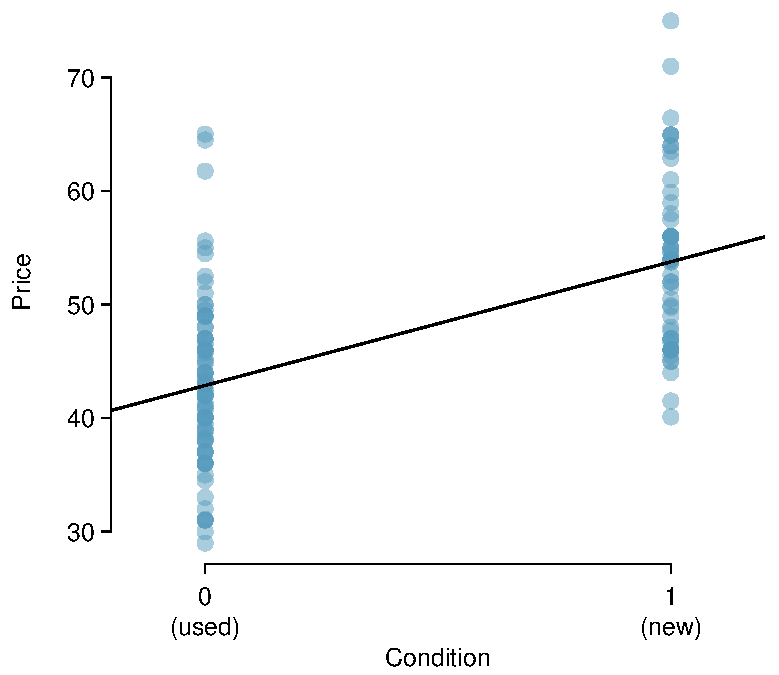
\includegraphics[width=0.725\textwidth]{ch_regr_mult_and_log/figures/marioKartSingle/marioKartSingle}
\caption{Scatterplot of the total auction price against the game's condition. The least squares line is also shown.}
\label{marioKartSingle}
\end{figure}

\begin{exercise}
Examine Figure~\ref{marioKartSingle}. Does the linear model seem reasonable?\footnote{Yes. Constant variability, nearly normal residuals, and linearity all appear reasonable.}
\end{exercise}

\textC{\pagebreak}

\begin{example}{Interpret the coefficient for the game's condition in the model. Is this coefficient significantly different from 0?}
Note that \var{cond\_\hspace{0.3mm}new} is a two-level categorical variable that takes value 1 when the game is new and value 0 when the game is used. So 10.90 means that the model predicts an extra \$10.90 for those games that are new versus those that are used. (See Section~\ref{categoricalPredictorsWithTwoLevels} for a review of the interpretation for two-level categorical predictor variables.) Examining the regression output in Table~\ref{singleVarModelsForPriceUsingCond}, we can see that the p-value for \var{cond\_\hspace{0.3mm}new} is very close to zero, indicating there is strong evidence that the coefficient is different from zero when using this simple one-variable model.
\end{example}

\subsection{Including and assessing many variables in a model}
\label{includingAndAssessingManyVariablesInAModel}

Sometimes there are underlying structures or relationships between predictor variables. For instance, new games sold on Ebay tend to come with more Wii wheels, which may have led to higher prices for those auctions. We would like to fit a model that includes all potentially important variables simultaneously. This would help us evaluate the relationship between a predictor variable and the outcome while controlling for the potential influence of other variables. This is the strategy used in \term{multiple regression}. While we remain cautious about making any causal interpretations using multiple regression, such models are a common first step in providing evidence of a causal connection.

\textC{\pagebreak}

We want to construct a model that accounts for not only the game condition, as in Section~\ref{twoSingleVariableModelsForMarioKartData}, but simultaneously accounts for three other variables: \var{stock\_\hspace{0.3mm}photo}, \var{duration}, and \var{wheels}.
\begin{align}
\widehat{\var{price}}
	&= \beta_0 + \beta_1\times \var{cond\_\hspace{0.3mm}new} +
		\beta_2\times \var{stock\_\hspace{0.3mm}photo} \notag \\
	&\qquad\  + \beta_3 \times  \var{duration} +
		\beta_4 \times  \var{wheels} \notag \\
\hat{y}
	&= \beta_0 + \beta_1 x_1 + \beta_2 x_2 +
		\beta_3 x_3 + \beta_4 x_4
\label{eqForMultipleRegrOfTotalPrForAllPredictors}
\end{align}
In this equation, $y$ represents the total price, $x_1$ indicates whether the game is new, $x_2$ indicates whether a stock photo was used, $x_3$ is the duration of the auction, and $x_4$ is the number of Wii wheels included with the game. Just as with the single predictor case, a multiple regression model may be missing important components or it might not precisely represent the relationship between the outcome and the available explanatory variables. While no model is perfect, we wish to explore the possibility that this one may fit the data reasonably well.

We estimate the parameters $\beta_0$, $\beta_1$, ..., $\beta_4$ in the same way as we did in the case of a single predictor. We select $b_0$, $b_1$, ..., $b_4$ that minimize the sum of the squared residuals:
\begin{align}\label{sumOfSqResInMultRegr}
SSE = e_1^2 + e_2^2 + \dots + e_{141}^2
	= \sum_{i=1}^{141} e_i^2
	 = \sum_{i=1}^{141} \left(y_i - \hat{y}_i\right)^2
\end{align}
Here there are 141 residuals, one for each observation. We typically use a computer to minimize the sum in Equation~\eqref{sumOfSqResInMultRegr} and compute point estimates, as shown in the sample output in Table~\ref{outputForMultipleRegrOutputForAllPredictors}. Using this output, we identify the point estimates $b_i$ of each $\beta_i$, just as we did in the one-predictor case.

\begin{table}[ht]
\centering
\begin{tabular}{rrrrr}
  \hline
  \vspace{-3.7mm} & & & & \\
 & Estimate & Std. Error & t value & Pr($>$$|$t$|$) \\ 
  \hline
  \vspace{-3.8mm} & & & & \\
(Intercept) & 36.2110 & 1.5140 & 23.92 & 0.0000 \\ 
  cond\_\hspace{0.3mm}new & 5.1306 & 1.0511 & 4.88 & 0.0000 \\ 
  stock\_\hspace{0.3mm}photo & 1.0803 & 1.0568 & 1.02 & 0.3085 \\ 
  duration & -0.0268 & 0.1904 & -0.14 & 0.8882 \\ 
  wheels & 7.2852 & 0.5547 & 13.13 & 0.0000 \\ 
   \hline
   &&&\multicolumn{2}{r}{$df=136$}
\end{tabular}
\caption{Output for the regression model where \var{price} is the outcome and \var{cond\_\hspace{0.3mm}new}, \var{stock\_\hspace{0.3mm}photo}, \var{duration}, and \var{wheels} are the predictors.}
\label{outputForMultipleRegrOutputForAllPredictors}
\end{table}
%library(openintro); library(xtable); data(marioKart); d <- marioKart[marioKart$totalPr < 100,]; d$cond <- relevel(d$cond, "used"); g <-lm(totalPr ~ cond + stockPhoto + duration + wheels, d)

\begin{termBox}{\tBoxTitle{Multiple regression model}
A multiple regression model is a linear model with many predictors. In general, we write the model as
\begin{align*}
\hat{y} = \beta_0 + \beta_1 x_1 + \beta_2 x_2 + \cdots + \beta_k x_k %+ \epsilon
\end{align*}
when there are $k$ predictors. We often estimate the $\beta_i$ parameters using a computer.\vspace{1mm}}
\end{termBox}

\textC{\pagebreak}

\begin{exercise} \label{eqForMultipleRegrOfTotalPrForAllPredictorsWithCoefficients}
Write out the model in Equation~\eqref{eqForMultipleRegrOfTotalPrForAllPredictors} using the point estimates from Table~\ref{outputForMultipleRegrOutputForAllPredictors}. How many predictors are there in this model?\footnote{$\hat{y} = 36.21 + 5.13x_1 + 1.08x_2 - 0.03x_3 + 7.29x_4$, and there are $k=4$ predictor variables.}
\end{exercise}

\begin{exercise}
What does $\beta_4$, the coefficient of variable $x_4$ (Wii wheels), represent? What is the point estimate of $\beta_4$?\footnote{It is the average difference in auction price for each additional Wii wheel included when holding the other variables constant. The point estimate is $b_4 = 7.29$.}
\end{exercise}

\begin{exercise} \label{computeMultipleRegressionResidualForMarioKart}
Compute the residual of the first observation in Table~\vref{marioKartDataMatrix} using the equation identified in Guided Practice~\ref{eqForMultipleRegrOfTotalPrForAllPredictorsWithCoefficients}.\footnote{$e_i = y_i - \hat{y_i} = 51.55 - 49.62 = 1.93$, where 49.62 was computed using the variables values from the observation and the equation identified in Guided Practice~\ref{eqForMultipleRegrOfTotalPrForAllPredictorsWithCoefficients}.}
\end{exercise}

\begin{example}{We estimated a coefficient for \var{cond\_\hspace{0.3mm}new} in Section~\ref{twoSingleVariableModelsForMarioKartData} of $b_1 = 10.90$ with a standard error of $SE_{b_1} = 1.26$ when using simple linear regression. Why might there be a difference between that estimate and the one in the multiple regression setting?} \label{colinearityOfCondNewAndStockPhoto}
If we examined the data carefully, we would see that some predictors are correlated. For instance, when we estimated the connection of the outcome \var{price} and predictor \var{cond\_\hspace{0.3mm}new} using simple linear regression, we were unable to control for other variables like the number of Wii wheels included in the auction. That model was biased by the confounding variable \var{wheels}. When we use both variables, this particular underlying and unintentional bias is reduced or eliminated (though bias from other confounding variables may still remain).
\end{example}

Example~\ref{colinearityOfCondNewAndStockPhoto} describes a common issue in multiple regression: correlation among predictor variables. We say the two predictor variables are \term{collinear} (pronounced as \emph{co-linear}) when they are correlated, and this collinearity complicates model estimation. While it is impossible to prevent collinearity from arising in observational data, experiments are usually designed to prevent predictors from being collinear.

\begin{exercise}
The estimated value of the intercept is 36.21, and one might be tempted to make some interpretation of this coefficient, such as, it is the model's predicted price when each of the variables take value zero: the game is used, the primary image is not a stock photo, the auction duration is zero days, and there are no wheels included. Is there any value gained by making this interpretation?\footnote{Three of the variables (\var{cond\_\hspace{0.3mm}new}, \var{stock\_\hspace{0.3mm}photo}, and \var{wheels}) do take value 0, but the auction duration is always one or more days. If the auction is not up for any days, then no one can bid on it! That means the total auction price would always be zero for such an auction; the interpretation of the intercept in this setting is not insightful.}
\end{exercise}


\subsection{Adjusted $R^2$ as a better estimate of explained variance}

\index{adjusted r squared@adjusted $R^2$ ($R_{adj}^2$)|(}

We first used $R^2$ in Section~\ref{fittingALineByLSR} to determine the amount of variability in the response that was explained by the model:
\begin{align*}
R^2 = 1 - \frac{\text{variability in residuals}}{\text{variability in the outcome}}
	= 1 - \frac{Var(e_i)}{Var(y_i)}
\end{align*}
where $e_i$ represents the residuals of the model and $y_i$ the outcomes. This equation remains valid in the multiple regression framework, but a small enhancement can often be even more informative.

\begin{exercise} \label{computeUnadjustedR2ForAllPredictorsInMarioKart}
The variance of the residuals for the model given in Guided Practice~\ref{computeMultipleRegressionResidualForMarioKart} is 23.34, and the variance of the total price in all the auctions is 83.06. Calculate $R^2$ for this model.\footnote{$R^2 = 1 - \frac{23.34}{83.06} = 0.719$.}
\end{exercise}

This strategy for estimating $R^2$ is acceptable when there is just a single variable. However, it becomes less helpful when there are many variables. The regular $R^2$ is a less estimate of the amount of variability explained by the model. To get a better estimate, we use the adjusted $R^2$.

\begin{termBox}{\tBoxTitle{Adjusted $\mathbf{R^2}$ as a tool for model assessment}
The \termsub{adjusted $\mathbf{R^2}$}{adjusted r squared@adjusted $R^2$ ($R_{adj}^2$)} is computed as
\begin{align*}
R_{adj}^{2} = 1-\frac{Var(e_i) / (n-k-1)}{Var(y_i) / (n-1)}
	= 1-\frac{Var(e_i)}{Var(y_i)} \times \frac{n-1}{n-k-1}
\end{align*}
where $n$ is the number of cases used to fit the model and $k$ is the number of predictor variables in the model.}
\end{termBox}

Because $k$ is never negative, the adjusted $R^2$ will be smaller -- often times just a little smaller -- than the unadjusted $R^2$. The reasoning behind the adjusted $R^2$ lies in the \termsub{degrees of freedom}{degrees of freedom (df)!regression} associated with each variance.\footnote{In multiple regression, the degrees of freedom associated with the variance of the estimate of the residuals is $n-k-1$, not $n-1$. For instance, if we were to make predictions for new data using our current model, we would find that the unadjusted $R^2$ is an overly optimistic estimate of the reduction in variance in the response, and using the degrees of freedom in the adjusted $R^2$ formula helps correct this bias.}

\begin{exercise}
There were $n=141$ auctions in the \data{mario\_\hspace{0.3mm}kart} data set and $k=4$ predictor variables in the model. Use $n$, $k$, and the variances from Guided Practice~\ref{computeUnadjustedR2ForAllPredictorsInMarioKart} to calculate $R_{adj}^2$ for the Mario Kart model.\footnote{$R_{adj}^2 = 1 - \frac{23.34}{83.06}\times \frac{141-1}{141-4-1} = 0.711$.}
\end{exercise}

\begin{exercise}
Suppose you added another predictor to the model, but the variance of the errors $Var(e_i)$ didn't go down. What would happen to the $R^2$? What would happen to the adjusted $R^2$?\hspace{0.7mm}\footnote{The unadjusted $R^2$ would stay the same and the adjusted $R^2$ would go down.}
\end{exercise}

Adjusted $R^2$ could have been used in Chapter~\ref{linRegrForTwoVar}. However, when there is only $k = 1$ predictors, adjusted $R^2$ is very close to regular $R^2$, so this nuance isn't typically important when considering only one predictor.

\index{adjusted r squared@adjusted $R^2$ ($R_{adj}^2$)|)}



\textC{\newpage}



%__________________
\section[Model selection]{Model selection \sectionvideohref{youtube-VB1qSwoF-l0&list=PLkIselvEzpM5f1HYzIjFt52SD4izsJ2_I}}
\label{introductionToMultipleRegression}


\label{modelSelection}

\index{model selection|(}

The best model is not always the most complicated. Sometimes including variables that are not evidently important can actually reduce the accuracy of predictions. In this section we discuss model selection strategies, which will help us eliminate variables from the model that are found to be less important.

In practice, the model that includes all available explanatory variables is often referred to as the \term{full model}. The full model may not be the best model, and if it isn't, we want to identify a smaller model that is preferable.


\subsection{Identifying variables in the model that may not be helpful}

Adjusted $R^2$ describes the strength of a model fit, and it is a useful tool for evaluating which predictors are adding value to the model, where \emph{adding value} means they are (likely) improving the accuracy in predicting future outcomes.

Let's consider two models, which are shown in Tables~\ref{outputForMultipleRegrOutputForAllPredictors2} and~\ref{marioKartMultipleRegressionModelAllButDuration}. The first table summarizes the full model since it includes all predictors, while the second does not include the \var{duration} variable.

\begin{table}[ht]
\centering
\begin{tabular}{rrrrr}
  \hline
  \vspace{-3.7mm} & & & & \\
 & Estimate & Std. Error & t value & Pr($>$$|$t$|$) \\ 
  \hline
  \vspace{-3.8mm} & & & & \\
(Intercept) & 36.2110 & 1.5140 & 23.92 & 0.0000 \\ 
  cond\_\hspace{0.3mm}new & 5.1306 & 1.0511 & 4.88 & 0.0000 \\ 
  stock\_\hspace{0.3mm}photo & 1.0803 & 1.0568 & 1.02 & 0.3085 \\ 
  duration & -0.0268 & 0.1904 & -0.14 & 0.8882 \\ 
  wheels & 7.2852 & 0.5547 & 13.13 & 0.0000 \\ 
   \hline
  \vspace{-3.6mm} & & & & \\
\multicolumn{3}{l}{$R_{adj}^2 = 0.7108$}&\multicolumn{2}{r}{$df=136$}
\end{tabular}
\caption{The fit for the full regression model, including the adjusted $R^2$.}
\label{outputForMultipleRegrOutputForAllPredictors2}
\end{table}

\begin{table}[ht]
\centering
\begin{tabular}{rrrrr}
  \hline
  \vspace{-3.7mm} & & & & \\
 & Estimate & Std. Error & t value & Pr($>$$|$t$|$) \\ 
  \hline
  \vspace{-3.8mm} & & & & \\
(Intercept) & 36.0483 & 0.9745 & 36.99 & 0.0000 \\ 
  cond\_\hspace{0.3mm}new & 5.1763 & 0.9961 & 5.20 & 0.0000 \\ 
  stock\_\hspace{0.3mm}photo & 1.1177 & 1.0192 & 1.10 & 0.2747 \\ 
  wheels & 7.2984 & 0.5448 & 13.40 & 0.0000 \\ 
   \hline
  \vspace{-3.6mm} & & & & \\
\multicolumn{3}{l}{$R_{adj}^2 = 0.7128$}&\multicolumn{2}{r}{$df=137$}
\end{tabular}
\caption{The fit for the regression model for predictors \var{cond\_new}, \var{stock\_photo}, and \var{wheels}.}
\label{marioKartMultipleRegressionModelAllButDuration}
\end{table}

\begin{example}{Which of the two models is better?}
We compare the adjusted $R^2$ of each model to determine which to choose. Since the first model has an $R^2_{adj}$ smaller than the $R^2_{adj}$ of the second model, we prefer the second model to the first.
\end{example}

Will the model without \var{duration} be better than the model with \var{duration}? We~cannot know for sure, but based on the adjusted $R^2$, this is our best assessment.


\subsection{Two model selection strategies}

Two common strategies for adding or removing variables in a multiple regression model are called \emph{backward elimination} and \emph{forward selection}. These techniques are often referred to as \term{stepwise} model selection strategies, because they add or delete one variable at a time as they ``step'' through the candidate predictors.

\termsub{Backward elimination}{backward elimination} starts with the model that includes all potential predictor variables. Variables are eliminated one-at-a-time from the model until we cannot improve the adjusted $R^2$. The strategy within each elimination step is to eliminate the variable that leads to the largest improvement in adjusted $R^2$.

\begin{example}{Results corresponding to the \emph{full model} for the \data{mario\_\hspace{0.3mm}kart} data are shown in Table~\ref{outputForMultipleRegrOutputForAllPredictors2}. How should we proceed under the backward elimination strategy?} \label{backwardEliminationExampleWMarioKartData}
Our baseline adjusted $R^2$ from the full model is $R^2_{adj} = 0.7108$, and we need to determine whether dropping a predictor will improve the adjusted $R^2$. To check, we fit four models that each drop a different predictor, and we record the adjusted $R^2$ from each:
\begin{center}
\begin{tabular}{lllll}
Exclude ... &
	\var{cond\_\hspace{0.3mm}new} &
	\var{stock\_\hspace{0.3mm}photo} &
	\var{duration} &
	\var{wheels} \\
&
	$R^2_{adj} = 0.6626$ &
	$R^2_{adj} = 0.7107$ &
	$R^2_{adj} = 0.7128$ &
	$R^2_{adj} = 0.3487$ \\
\end{tabular}
\end{center}
The third model without \var{duration} has the highest adjusted $R^2$ of 0.7128, so we compare it to the adjusted $R^2$ for the full model. Because eliminating \var{duration} leads to a model with a higher adjusted $R^2$, we drop \var{duration} from the model.

Since we eliminated a predictor from the model in the first step, we see whether we should eliminate any additional predictors. Our baseline adjusted $R^2$ is now $R^2_{adj} = 0.7128$. We now fit three new models, which consider eliminating each of the three remaining predictors:
\begin{center}
\begin{tabular}{llll}
Exclude \var{duration} and ... &
	\var{cond\_\hspace{0.3mm}new} &
	\var{stock\_\hspace{0.3mm}photo} &
	\var{wheels} \\
&
	$R^2_{adj} = 0.6587$ &
	$R^2_{adj} = 0.7124$ &
	$R^2_{adj} = 0.3414$ \\
\end{tabular}
\end{center}
None of these models lead to an improvement in adjusted $R^2$, so we do not eliminate any of the remaining predictors. That is, after backward elimination, we are left with the model that keeps \var{cond\_\hspace{0.3mm}new}, \var{stock\_\hspace{0.3mm}photos}, and \var{wheels}, which we can summarize using the coefficients from Table~\ref{marioKartMultipleRegressionModelAllButDuration}:
\begin{align*}
\hat{y} \ &= \ b_0 + b_1x_1 + b_2x_2 + b_4x_4 \\
\widehat{price} &= \ 36.05 + 5.18 \times \text{\var{cond\_\hspace{0.3mm}new}} + 1.12 \times \text{\var{stock\_\hspace{0.3mm}photo}} + 7.30 \times \text{\var{wheels}}
\end{align*}
\end{example}

\textC{\newpage}

The \term{forward selection} strategy is the reverse of the backward elimination technique. Instead of eliminating variables one-at-a-time, we add variables one-at-a-time until we cannot find any variables that improve the model (as measured by adjusted $R^2$).

\begin{example}{Construct a model for the \data{mario\_\hspace{0.3mm}kart} data set using the forward selection strategy.}\label{forwardEliminationExampleWMarioKartData}
We start with the model that includes no variables. Then we fit each of the possible models with just one variable. That is, we fit the model including just \var{cond\_\hspace{0.3mm}new}, then the model including just \var{stock\_\hspace{0.3mm}photo}, then a model with just \var{duration}, and a model with just \var{wheels}. Each of the four models provides an adjusted $R^2$ value:
\begin{center}
\begin{tabular}{lllll}
Add ... &
	\var{cond\_\hspace{0.3mm}new} &
	\var{stock\_\hspace{0.3mm}photo} &
	\var{duration} &
	\var{wheels} \\
&
	$R^2_{adj} = 0.3459$ &
	$R^2_{adj} = 0.0332$ &
	$R^2_{adj} = 0.1338$ &
	$R^2_{adj} = 0.6390$ \\
\end{tabular}
\end{center}
In this first step, we compare the adjusted $R^2$ against a baseline model that has no predictors. The no-predictors model always has $R_{adj}^2 = 0$. The model with one predictor that has the largest adjusted $R^2$ is the model with the \var{wheels} predictor, and because this adjusted $R^2$ is larger than the adjusted $R^2$ from the model with no predictors ($R_{adj}^2 = 0$), we will add this variable to our model.

We repeat the process again, this time considering 2-predictor models where one of the predictors is \var{wheels} and with a new baseline of $R^2_{adj} = 0.6390$:
\begin{center}
\begin{tabular}{llll}
Add \var{wheels} and ... &
	\var{cond\_\hspace{0.3mm}new} &
	\var{stock\_\hspace{0.3mm}photo} &
	\var{duration} \\
&
	$R^2_{adj} = 0.7124$ &
	$R^2_{adj} = 0.6587$ &
	$R^2_{adj} = 0.6528$ \\
\end{tabular}
\end{center}
The best predictor in this stage, \var{cond\_\hspace{0.3mm}new}, has a higher adjusted $R^2$ (0.7124) than the baseline (0.6390), so we also add \var{cond\_\hspace{0.3mm}new} to the model.

Since we have again added a variable to the model, we continue and see whether it would be beneficial to add a third variable:
\begin{center}
\begin{tabular}{lll}
Add \var{wheels}, \var{cond\_\hspace{0.3mm}new}, and ... &
	\var{stock\_\hspace{0.3mm}photo} &
	\var{duration} \\
&
	$R^2_{adj} = 0.7128$ &
	$R^2_{adj} = 0.7107$ \\
\end{tabular}
\end{center}
The model adding \var{stock\_\hspace{0.3mm}photo} improved adjusted $R^2$ (0.7124 to 0.7128), so we add \var{stock\_\hspace{0.3mm}photo} to the model.

Because we have again added a predictor, we check whether adding the last variable, \var{duration}, will improve adjusted $R^2$. We compare the adjusted $R^2$ for the model with \var{duration} and the other three predictors (0.7108) to the model that only considers \var{wheels}, \var{cond\_\hspace{0.3mm}new}, and \var{stock\_\hspace{0.3mm}photo} (0.7128). Adding \var{duration} does not improve the adjusted $R^2$, so we do not add it to the model, and we have arrived at the same model that we identified from backward elimination.

\end{example}

\begin{termBox}{\tBoxTitle{Model selection strategies}
Backward elimination begins with the largest model and eliminates variables one-by-one until we are satisfied that all remaining variables are important to the model. Forward selection starts with no variables included in the model, then it adds in variables according to their importance until no other important variables are found.}
\end{termBox}

There is no guarantee that backward elimination and forward selection will arrive at the same final model. If both techniques are tried and they arrive at different models, we choose the model with the larger $R_{adj}^2$; other tie-break options exist but are beyond the scope of this book.



\subsection{The p-value approach, an alternative to adjusted $R^2$}

The p-value may be used as an alternative to adjusted $R^2$ for model selection.

In backward elimination, we would identify the predictor corresponding to the largest p-value. If the p-value is above the significance level, usually $\alpha = 0.05$, then we would drop that variable, refit the model, and repeat the process. If the largest p-value is less than $\alpha = 0.05$, then we would not eliminate any predictors and the current model would be our best-fitting model.

In forward selection with p-values, we reverse the process. We begin with a model that has no predictors, then we fit a model for each possible predictor, identifying the model where the corresponding predictor's p-value is smallest. If that p-value is smaller than $\alpha = 0.05$, we add it to the model and repeat the process, considering whether to add more variables one-at-a-time. When none of the remaining predictors can be added to the model and have a p-value less than 0.05, then we stop adding variables and the current model would be our best-fitting model.

\begin{exercise}
Examine Table~\ref{marioKartMultipleRegressionModelAllButDuration} on page~\pageref{marioKartMultipleRegressionModelAllButDuration}, which considers the model including the \var{cond\_\hspace{0.3mm}new}, \var{stock\_\hspace{0.3mm}photo}, and \var{wheels} predictors. If we were using the p-value approach with backward elimination and we were considering this model, which of these three variables would be up for elimination? Would we drop that variable, or would we keep it in the model?\footnote{The \var{stock\_\hspace{0.3mm}photo} predictor is up for elimination since it has the largest p-value. Additionally, since that p-value is larger than 0.05, we would in fact eliminate \var{stock\_\hspace{0.3mm}photo} from the model.}
\end{exercise}

While the adjusted $R^2$ and p-value approaches are similar, they sometimes lead to different models, with the adjusted $R^2$ approach tending to include more predictors in the final model. For example, if we had used the p-value approach with the auction data, we would not have included the \var{stock\_\hspace{0.3mm}photo} predictor in the final model.

\begin{tipBox}{\tBoxTitle{When to use the adjusted $R^2$ and when to use the p-value approach}
When the sole goal is to improve prediction accuracy, use adjusted $R^2$. This is commonly the case in machine learning applications.\\[-2mm]

When we care about understanding which variables are statistically significant predictors of the response, or if there is interest in producing a simpler model at the potential cost of a little prediction accuracy, then the p-value approach is preferred.}
\end{tipBox}

Regardless of whether you use adjusted $R^2$ or the p-value approach, or if you use the backward elimination of forward selection strategy, our job is not done after variable selection. We must still verify the model conditions are reasonable.

\index{model selection|)}



%%%%%
\section[Checking model assumptions using graphs]{Checking model assumptions using graphs \sectionvideohref{youtube-3KSUeYMKt5A&list=PLkIselvEzpM5f1HYzIjFt52SD4izsJ2_I}}
\label{multipleRegressionModelAssumptions}

\index{multiple regression!model assumptions|(}

Multiple regression methods using the model
\begin{align*}
\hat{y} &= \beta_0 + \beta_1x_1 + \beta_2x_2 + \cdots + \beta_kx_k
\end{align*}
generally depend on the following four assumptions:
\begin{enumerate}
\setlength{\itemsep}{0mm}
\item the residuals of the model are nearly normal,
\item the variability of the residuals is nearly constant,
\item the residuals are independent, and
\item each variable is linearly related to the outcome.
\end{enumerate}
\termsub{Diagnostic plots}{diagnostic plots} can be used to check each of these assumptions. We will consider the model from the Mario Kart auction data, and check whether there are any notable concerns:
\begin{align*}
\widehat{price} &= \ 36.05 + 5.18 \times \text{\var{cond\_\hspace{0.3mm}new}} + 1.12 \times \text{\var{stock\_\hspace{0.3mm}photo}} + 7.30 \times \text{\var{wheels}}
\end{align*}

\begin{description}
\item[Normal probability plot.] A normal probability plot of the residuals is shown in Figure~\ref{mkDiagnosticNormalQuantilePlot}. While the plot exhibits some minor irregularities, there are no outliers that might be cause for concern. In a normal probability plot for residuals, we tend to be most worried about residuals that appear to be outliers, since these indicate long tails in the distribution of residuals.

\begin{figure}[h]
\centering
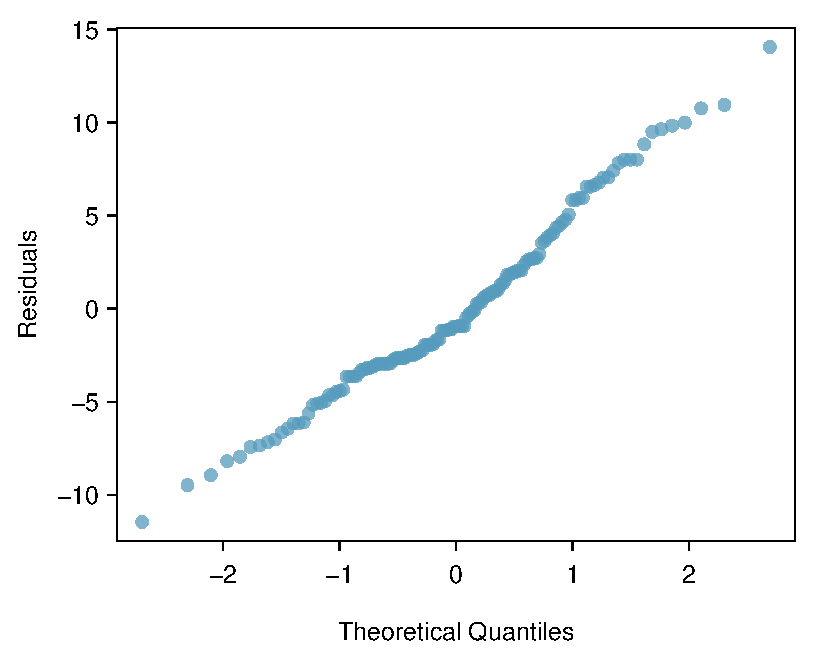
\includegraphics[width=0.71\textwidth]{ch_regr_mult_and_log/figures/marioKartDiagnostics/mkDiagnosticNormalQuantilePlot}
\caption{A normal probability plot of the residuals is helpful in identifying observations that might be outliers.}
\label{mkDiagnosticNormalQuantilePlot}
\end{figure}

\item[Absolute values of residuals against fitted values.] A plot of the absolute value of the residuals against their corresponding fitted values ($\hat{y}_i$) is shown in Figure~\ref{mkDiagnosticEvsAbsF}. This plot is helpful to check the condition that the variance of the residuals is approximately constant. We don't see any obvious deviations from constant variance in this example.

\begin{figure}
\centering
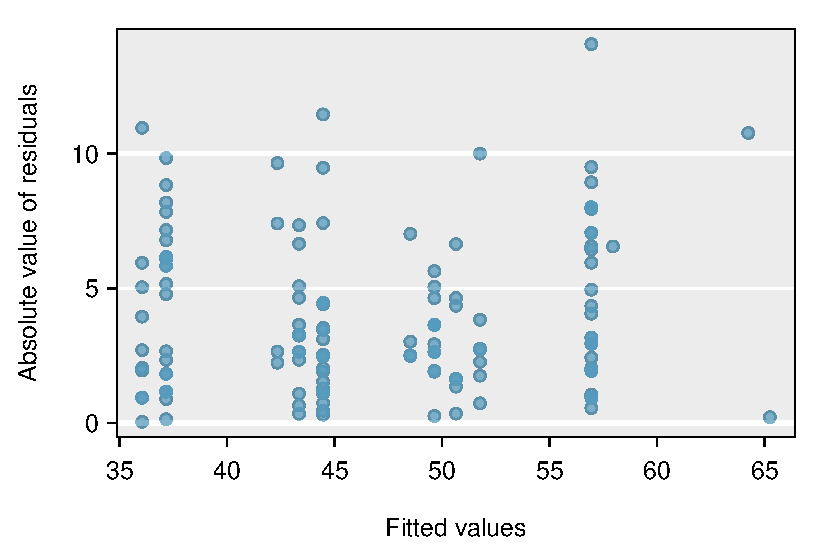
\includegraphics[width=0.7\textwidth]{ch_regr_mult_and_log/figures/marioKartDiagnostics/mkDiagnosticEvsAbsF}
\caption{Comparing the absolute value of the residuals against the fitted values ($\hat{y}_i$) is helpful in identifying deviations from the constant variance assumption.}
\label{mkDiagnosticEvsAbsF}
\end{figure}

\item[Residuals in order of their data collection.] A plot of the residuals in the order their corresponding auctions were observed is shown in Figure~\ref{mkDiagnosticInOrder}. Such a plot is helpful in identifying any connection between cases that are close to one another, e.g. we could look for declining prices over time or if there was a time of the day when auctions tended to fetch a higher price. Here we see no structure that indicates a problem.\footnote{An especially rigorous check would use \term{time series} methods. For instance, we could check whether consecutive residuals are correlated. Doing so with these residuals yields no statistically significant correlations.}

\begin{figure}[h]
\centering
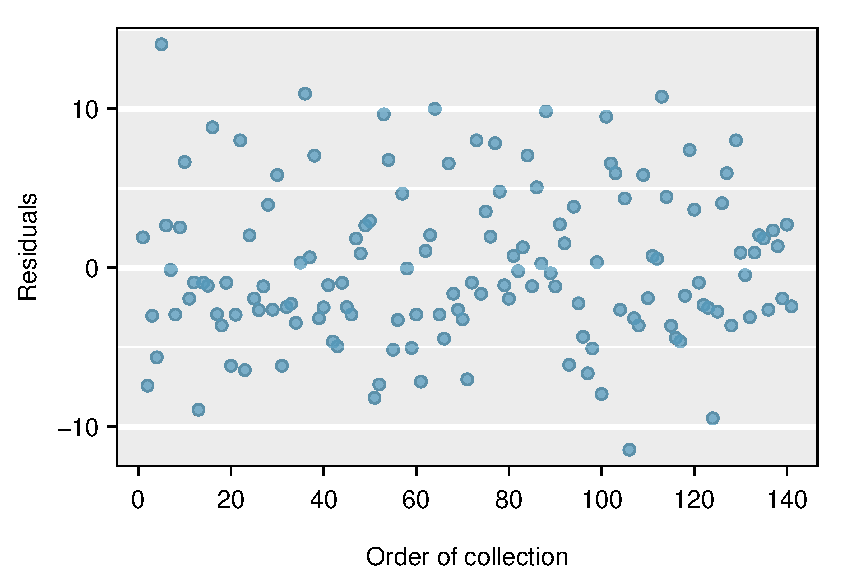
\includegraphics[width=0.72\textwidth]{ch_regr_mult_and_log/figures/marioKartDiagnostics/mkDiagnosticInOrder}
\caption{Plotting residuals in the order that their corresponding observations were collected helps identify connections between successive observations. If it seems that consecutive observations tend to be close to each other, this indicates the independence assumption of the observations would fail.}
\label{mkDiagnosticInOrder}
\end{figure}

\item[Residuals against each predictor variable.] We consider a plot of the residuals against the \var{cond\_\hspace{0.3mm}new} variable, the residuals against the \var{stock\_\hspace{0.3mm}photo} variable, and the residuals against the \var{wheels} variable. These plots are shown in Figure~\ref{mkDiagnosticEvsVariables}. For the two-level condition variable, we are guaranteed not to see any remaining trend, and instead we are checking that the variability doesn't fluctuate across groups, which it does not. However, looking at the stock photo variable, we find that there is some difference in the variability of the residuals in the two groups. Additionally, when we consider the residuals against the \var{wheels} variable, we see some possible structure. There appears to be curvature in the residuals, indicating the relationship is probably not linear.

\begin{figure}
\centering
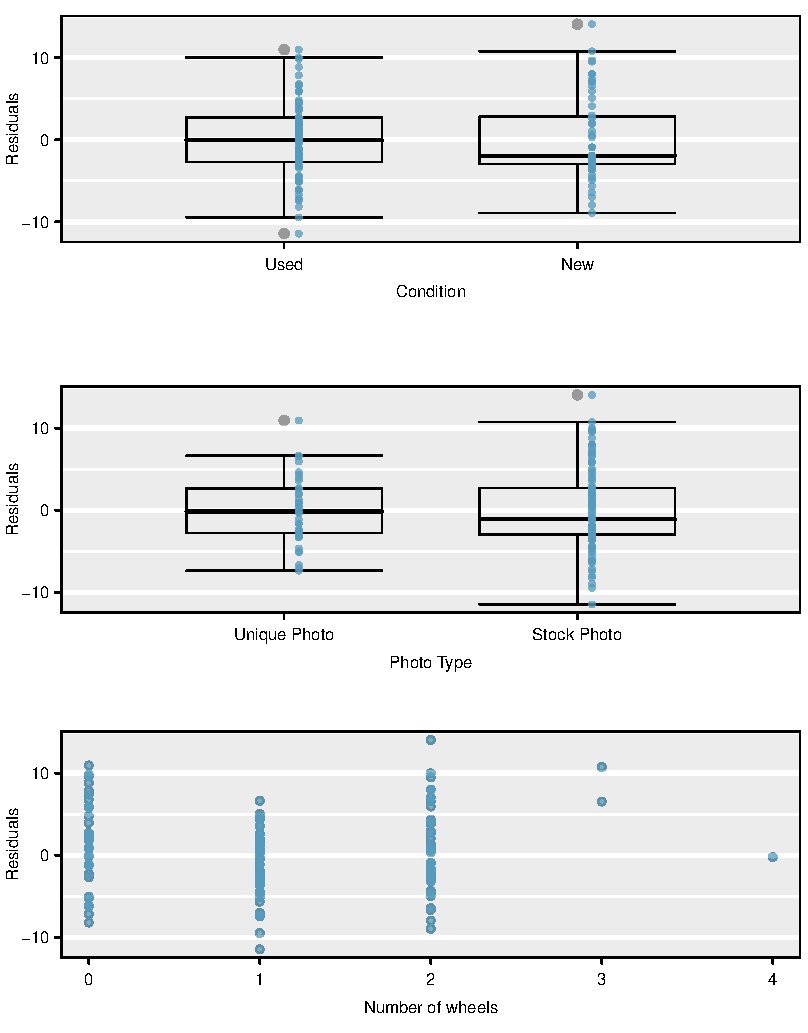
\includegraphics[width=\textwidth]{ch_regr_mult_and_log/figures/marioKartDiagnostics/mkDiagnosticEvsVariables}
\caption{For the condition and stock photo variables, we check for differences in the distribution shape or variability of the residuals. In the case of the stock photos variable, we see a little less variability in the unique photo group than the stock photo group. For numerical predictors, we also check for trends or other structure. We see some slight bowing in the residuals against the \var{wheels} variable in the bottom plot.}
\label{mkDiagnosticEvsVariables}
\end{figure}

\end{description}

It is necessary to summarize diagnostics for any model fit. If the diagnostics support the model assumptions, this would improve credibility in the findings. If the diagnostic assessment shows remaining underlying structure in the residuals, we should try to adjust the model to account for that structure. If we are unable to do so, we may still report the model but must also note its shortcomings. In the case of the auction data, we report that there appears to be non-constant variance in the stock photo variable and that there may be a nonlinear relationship between the total price and the number of wheels included for an auction. This information would be important to buyers and sellers who may review the analysis, and omitting this information could be a setback to the very people who the model might assist.

\begin{tipBox}{\tipBoxTitle[]{``All models are wrong, but some are useful'' -George E.P. Box}
The truth is that no model is perfect. However, even imperfect models can be useful. Reporting a flawed model can be reasonable so long as we are clear and report the model's shortcomings.}
\end{tipBox}

\begin{caution}
{Don't report results when assumptions are grossly violated}
{While there is a little leeway in model assumptions, don't go too far. If model assumptions are very clearly violated, consider a new model, even if it means learning more statistical methods or hiring someone who can help.}
\end{caution}

\begin{tipBox}{\tipBoxTitle{Confidence intervals in multiple regression}
\index{confidence interval}
Confidence intervals for coefficients in multiple regression can be computed using the same formula as in the single predictor model:
\begin{align*}
b_i \ \pm\ t_{df}^{\star}SE_{b_{i}}
\end{align*}
where $t_{df}^{\star}$ is the appropriate $t$-value corresponding to the confidence level and model degrees of freedom, $df=n-k-1$.}
\index{multiple regression!model assumptions|)}
\index{data!mario\_kart|)}
\index{multiple regression|)}
\end{tipBox}


%__________________
\section[Introduction to logistic regression]{Introduction to logistic regression \sectionvideohref{youtube-uYC2eLVSpI8&list=PLkIselvEzpM5f1HYzIjFt52SD4izsJ2_I}}
\label{logisticRegression}

\index{logistic regression|(}

In this section we introduce \term{logistic regression} as a tool for building models when there is a categorical response variable with two levels. Logistic regression is a type of \term{generalized linear model} (GLM) for response variables where regular multiple regression does not work very well. In particular, the response variable in these settings often takes a form where residuals look completely different from the normal distribution.

GLMs can be thought of as a two-stage modeling approach. We first model the response variable using a probability distribution, such as the binomial or Poisson distribution. Second, we model the parameter of the distribution using a collection of predictors and a special form of multiple regression.

\index{data!email|(}

In Section~\ref{logisticRegression} we will revisit the \data{email} data set from Chapter~\ref{introductionToData}. These emails were collected from a single email account, and we will work on developing a basic spam filter using these data. The response variable, \var{spam}, has been encoded to take value~0 when a message is not spam and~1 when it is spam. Our task will be to build an appropriate model that classifies messages as spam or not spam using email characteristics coded as predictor variables. While this model will not be the same as those used in large-scale spam filters, it shares many of the same features. 

\subsection{Email data}

The \data{email} data set was first presented in Chapter~\ref{introductionToData} with a relatively small number of variables. In fact, there are many more variables available that might be useful for classifying spam. Descriptions of these variables are presented in Table~\ref{emailVariables}. The \var{spam} variable will be the outcome, and the other 10 variables will be the model predictors. While we have limited the predictors used in this section to be categorical variables (where many are represented as indicator variables), numerical predictors may also be used in logistic regression. See the footnote for an additional discussion on this topic.\footnote{Recall from Chapter~\ref{linRegrForTwoVar} that if outliers are present in predictor variables, the corresponding observations may be especially influential on the resulting model. This is the motivation for omitting the numerical variables, such as the number of characters and line breaks in emails, that we saw in Chapter~\ref{introductionToData}. These variables exhibited extreme skew. We could resolve this issue by transforming these variables (e.g. using a log-transformation), but we will omit this further investigation for brevity.}

\begin{table}
\centering\small
\begin{tabular}{lp{10.5cm}}
\hline
{\bf variable} & {\bf description} \\
\hline
\var{spam} & Specifies whether the message was spam. \\
\var{to\_\hspace{0.3mm}multiple} & An indicator variable for if more than one person was listed in the \emph{To} field of the email.  \\
\var{cc} & An indicator for if someone was CCed on the email. \\
\var{attach} & An indicator for if there was an attachment, such as a document or image.   \\
\var{dollar} & An indicator for if the word ``dollar'' or dollar symbol (\$) appeared in the email.  \\
\var{winner} & An indicator for if the word ``winner'' appeared in the email message.  \\
\var{inherit} & An indicator for if the word ``inherit'' (or a variation, like ``inheritance'') appeared in the email.  \\
\var{password} & An indicator for if the word ``password'' was present in the email.  \\
\var{format} & Indicates if the email contained special formatting, such as bolding, tables, or links    \\
\var{re\_\hspace{0.3mm}subj} & Indicates whether ``Re:'' was included at the start of the email subject.   \\
\var{exclaim\_\hspace{0.3mm}subj} & Indicates whether any exclamation point was included in the email subject.    \\
\hline
\end{tabular}
\caption{Descriptions for 11 variables in the \data{email} data set. Notice that all of the variables are indicator\index{indicator variable} variables, which take the value 1 if the specified characteristic is present and 0 otherwise.}
\label{emailVariables}
\end{table}


\subsection{Modeling the probability of an event}
\label{modelingTheProbabilityOfAnEvent}

\begin{tipBox}{\tipBoxTitle{Notation for a logistic regression model}
The outcome variable for a GLM is denoted by $Y_i$, where the index $i$ is used to represent observation $i$. In the email application, $Y_i$ will be used to represent whether email $i$ is spam ($Y_i=1$) or not ($Y_i=0$). \vspace{3mm}

The predictor variables are represented as follows: $x_{1,i}$ is the value of variable 1 for observation $i$, $x_{2,i}$ is the value of variable 2 for observation $i$, and so on.}
\end{tipBox}

Logistic regression is a generalized linear model where the outcome is a two-level categorical variable. The outcome, $Y_i$, takes the value 1 (in our application, this represents a spam message) with probability $p_i$ and the value 0 with probability $1-p_i$. It~is the probability $p_i$ that we model in relation to the predictor variables.

The logistic regression model relates the probability an email is spam ($p_i$) to the predictors $x_{1,i}$, $x_{2,i}$, ..., $x_{k,i}$ through a framework much like that of multiple regression:
\begin{align}
transformation(p_{i}) = \beta_0 + \beta_1x_{1,i} + \beta_2 x_{2,i} + \cdots \beta_k x_{k,i}
\label{linkTransformationEquation}
\end{align}
We want to choose a transformation in Equation~\eqref{linkTransformationEquation} that makes practical and mathematical sense. For example, we want a transformation that makes the range of possibilities on the left hand side of Equation~\eqref{linkTransformationEquation} equal to the range of possibilities for the right hand side; if there was no transformation for this equation, the left hand side could only take values between 0 and 1, but the right hand side could take values outside of this range. A common transformation for $p_i$ is the \term{logit transformation}, which may be written as
\begin{align*}
logit(p_i) = \log_{e}\left( \frac{p_i}{1-p_i} \right)
\end{align*}
The logit transformation is shown in Figure~\ref{logitTransformationFigureHoriz}. Below, we rewrite Equation~\eqref{linkTransformationEquation} using the logit transformation of $p_i$:
\begin{align*}
\log_{e}\left( \frac{p_i}{1-p_i} \right)
	= \beta_0 + \beta_1 x_{1,i} + \beta_2 x_{2,i} + \cdots + \beta_k x_{k,i}
\end{align*}
In our spam example, there are 10 predictor variables, so $k = 10$. This model isn't very intuitive, but it still has some resemblance to multiple regression, and we can fit this model using software. In fact, once we look at results from software, it will start to feel like we're back in multiple regression, even if the interpretation of the coefficients is more complex.

\textC{\newpage}

\begin{figure}
\centering
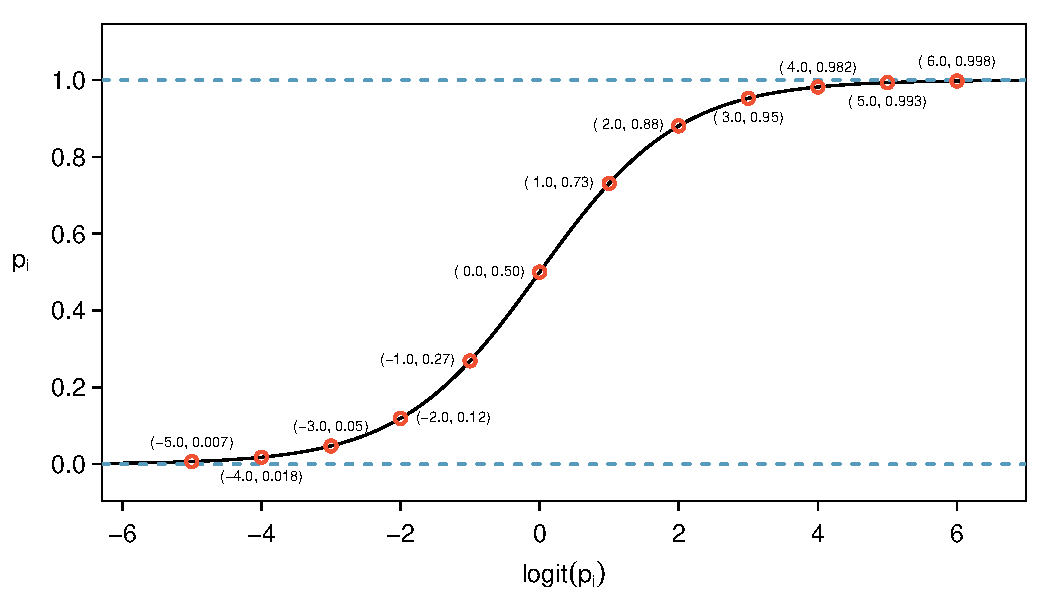
\includegraphics[width=\textwidth]{ch_regr_mult_and_log/figures/logitTransformationFigureHoriz/logitTransformationFigureHoriz}
\caption{Values of $p_i$ against values of $logit(p_i)$.}
\label{logitTransformationFigureHoriz}
\end{figure}

\begin{example}{Here we create a spam filter with a single predictor: \var{to\_\hspace{0.3mm}multiple}. This variable indicates whether more than one email address was listed in the \emph{To} field of the email. The following logistic regression model was fit using statistical software:
\begin{align*}
\log\left( \frac{p_i}{1-p_i} \right) = -2.12 - 1.81\times\text{\var{to\_\hspace{0.3mm}multiple}}
\end{align*}
%library(openintro); data(email); tm <- email$to_multiple > 0; g <- glm(email$spam ~ tm, family=binomial); summary(g); a <- exp(-2.12); a/(1+a); a <- exp(-2.12-1.81); a/(1+a)
If an email is randomly selected and it has just one address in the \emph{To} field, what is the probability it is spam? What if more than one address is listed in the \emph{To} field?}\label{logisticExampleWithToMultiple}
If there is only one email in the \emph{To} field, then \var{to\_\hspace{0.3mm}multiple} takes value 0 and the right side of the model equation equals -2.12. Solving for $p_i$: $\frac{e^{-2.12}}{1 + e^{-2.12}} = 0.11$. Just as we labeled a fitted value of $y_i$ with a ``hat'' in single-variable and multiple regression, we will do the same for this probability: $\hat{p}_i = 0.11$.

If there is more than one address listed in the \emph{To} field, then the right side of the model equation is $-2.12 - 1.81\times1 = -3.93$, which corresponds to a probability $\hat{p}_i = 0.02$.

Notice that we could examine -2.12 and -3.93 in Figure~\ref{logitTransformationFigureHoriz} to estimate the probability before formally calculating the value.
\end{example}

To convert from values on the regression-scale (e.g. -2.12 and -3.93 in Example~\ref{logisticExampleWithToMultiple}), use the following formula, which is the result of solving for $p_i$ in the regression model:
\begin{align*}
p_i
	= \frac{e^{\beta_0 + \beta_1 x_{1,i}+\cdots+\beta_k x_{k,i}}}
		{\ 1\ \ +\ \ e^{\beta_0 + \beta_1 x_{1,i}+\cdots+\beta_k x_{k,i}}\ }
\end{align*}
As with most applied data problems, we substitute the point estimates for the parameters (the $\beta_i$) so that we may make use of this formula. In Example~\ref{logisticExampleWithToMultiple}, the probabilities were calculated as
\begin{align*}
&\frac{\ e^{-2.12}\ }{\ 1\ +\ e^{-2.12}\ } = 0.11 && \frac{\ e^{-2.12 - 1.81}\ }{\ 1\ +\ e^{-2.12 - 1.81}\ } = 0.02
\end{align*}
While the information about whether the email is addressed to multiple people is a helpful start in classifying email as spam or not, the probabilities of 11\% and 2\% are not dramatically different, and neither provides very strong evidence about which particular email messages are spam. To get more precise estimates, we'll need to include many more variables in the model.

We used statistical software to fit the logistic regression model with all ten predictors described in Table~\ref{emailVariables}. Like multiple regression, the result may be presented in a summary table, which is shown in Table~\ref{emailLogisticModelResults}. The structure of this table is almost identical to that of multiple regression; the only notable difference is that the p-values are calculated using the normal distribution rather than the $t$-distribution.

\begin{table}[ht]
\centering
\begin{tabular}{rrrrr}
  \hline
  \vspace{-3.7mm} & & & & \\
 & Estimate & Std. Error & z value & Pr($>$$|$z$|$) \\ 
  \hline
  \vspace{-3.8mm} & & & & \\
(Intercept) & -0.8362 & 0.0962 & -8.69 & 0.0000 \\ 
  to\_\hspace{0.3mm}multiple & -2.8836 & 0.3121 & -9.24 & 0.0000 \\ 
  winner & 1.7038 & 0.3254 & 5.24 & 0.0000 \\ 
  format & -1.5902 & 0.1239 & -12.84 & 0.0000 \\ 
  re\_\hspace{0.3mm}subj & -2.9082 & 0.3708 & -7.84 & 0.0000 \\ 
  exclaim\_\hspace{0.3mm}subj & 0.1355 & 0.2268 & 0.60 & 0.5503 \\ 
  cc & -0.4863 & 0.3054 & -1.59 & 0.1113 \\ 
  attach & 0.9790 & 0.2170 & 4.51 & 0.0000 \\ 
  dollar & -0.0582 & 0.1589 & -0.37 & 0.7144 \\ 
  inherit & 0.2093 & 0.3197 & 0.65 & 0.5127 \\ 
  password & -1.4929 & 0.5295 & -2.82 & 0.0048 \\ 
\hline
\end{tabular}
\caption{Summary table for the full logistic regression model for the spam filter example.}
\label{emailLogisticModelResults}
\end{table}
% library(openintro); ?email # run example
% library(xtable); xtable(g)

Just like multiple regression, we could trim some variables from the model using the p-value. Using backward elimination with a p-value cutoff of 0.05 (start with the full model and trim the predictors with p-values greater than 0.05), we ultimately eliminate the \var{exclaim\_\hspace{0.3mm}subj}, \var{dollar}, \var{inherit}, and \var{cc} predictors. The remainder of this section will rely on this smaller model, which is summarized in Table~\ref{emailLogisticReducedModel}.

\begin{table}[ht]
\centering
\begin{tabular}{rrrrr}
  \hline
  \vspace{-3.7mm} & & & & \\
 & Estimate & Std. Error & z value & Pr($>$$|$z$|$) \\ 
  \hline
  \vspace{-3.8mm} & & & & \\
(Intercept) & -0.8595 & 0.0910 & -9.44 & 0.0000 \\ 
  to\_\hspace{0.3mm}multiple & -2.8372 & 0.3092 & -9.18 & 0.0000 \\ 
  winner & 1.7370 & 0.3218 & 5.40 & 0.0000 \\ 
  format & -1.5569 & 0.1207 & -12.90 & 0.0000 \\ 
  re\_\hspace{0.3mm}subj & -3.0482 & 0.3630 & -8.40 & 0.0000 \\ 
  attach & 0.8643 & 0.2042 & 4.23 & 0.0000 \\ 
  password & -1.4871 & 0.5290 & -2.81 & 0.0049 \\ 
\hline
\end{tabular}
\caption{Summary table for the logistic regression model for the spam filter, where variable selection has been performed.}
\label{emailLogisticReducedModel}
\end{table}
% library(openintro); ?email # run example
% g <- glm(spam ~ to_multiple + winner + format + re_subj + attach + password, data=e, family=binomial); xtable(g)

\textC{\pagebreak}

\begin{exercise}
Examine the summary of the reduced model in Table~\ref{emailLogisticReducedModel}, and in particular, examine the \var{to\_\hspace{0.3mm}multiple} row. Is the point estimate the same as we found before, -1.81, or is it different? Explain why this might be.\footnote{The new estimate is different: -2.87. This new value represents the estimated coefficient when we are also accounting for other variables in the logistic regression model.}
\end{exercise}

Point estimates will generally change a little -- and sometimes a lot -- depending on which other variables are included in the model. This is usually due to colinearity in the predictor variables. We previously saw this in the Ebay auction example when we compared the coefficient of \var{cond\_\hspace{0.3mm}new} in a single-variable model and the corresponding coefficient in the multiple regression model that used three additional variables (see Sections~\ref{twoSingleVariableModelsForMarioKartData} and~\ref{includingAndAssessingManyVariablesInAModel}).

\begin{example}{Spam filters are built to be automated, meaning a piece of software is written to collect information about emails as they arrive, and this information is put in the form of variables. These variables are then put into an algorithm that uses a statistical model, like the one we've fit, to classify the email. Suppose we write software for a spam filter using the reduced model shown in Table~\ref{emailLogisticReducedModel}. If an incoming email has the word ``winner'' in it, will this raise or lower the model's calculated probability that the incoming email is spam?} \label{exampleForSpamAndWinner}
The estimated coefficient of \var{winner} is positive (1.7370). A positive coefficient estimate in logistic regression, just like in multiple regression, corresponds to a positive association between the predictor and response variables when accounting for the other variables in the model. Since the response variable takes value 1 if an email is spam and 0 otherwise, the positive coefficient indicates that the presence of ``winner'' in an email raises the model probability that the message is spam.
\end{example}

\begin{example}{Suppose the same email from Example~\ref{exampleForSpamAndWinner} was in HTML format, meaning the \var{format} variable took value 1. Does this characteristic increase or decrease the probability that the email is spam according to the model?}\label{exampleForSpamAndFormat}
Since HTML corresponds to a value of 1 in the \var{format} variable and the coefficient of this variable is negative (-1.5569), this would lower the probability estimate returned from the model.
\end{example}

\subsection{Practical decisions in the email application}

Examples~\ref{exampleForSpamAndWinner} and~\ref{exampleForSpamAndFormat} highlight a key feature of logistic and multiple regression. In the spam filter example, some email characteristics will push an email's classification in the direction of spam while other characteristics will push it in the opposite direction.

If we were to implement a spam filter using the model we have fit, then each future email we analyze would fall into one of three categories based on the email's characteristics:
\begin{enumerate}
\item The email characteristics generally indicate the email is not spam, and so the resulting probability that the email is spam is quite low, say, under 0.05.
\item The characteristics generally indicate the email is spam, and so the resulting probability that the email is spam is quite large, say, over 0.95.
\item The characteristics roughly balance each other out in terms of evidence for and against the message being classified as spam. Its probability falls in the remaining range, meaning the email cannot be adequately classified as spam or not spam.
\end{enumerate}
If we were managing an email service, we would have to think about what should be done in each of these three instances. In an email application, there are usually just two possibilities: filter the email out from the regular inbox and put it in a ``spambox'', or let the email go to the regular inbox.

\begin{exercise}
The first and second scenarios are intuitive. If the evidence strongly suggests a message is not spam, send it to the inbox. If the evidence strongly suggests the message is spam, send it to the spambox. How should we handle emails in the third category?\footnote{In this particular application, we should err on the side of sending more mail to the inbox rather than mistakenly putting good messages in the spambox. So, in summary: emails in the first and last categories go to the regular inbox, and those in the second scenario go to the spambox.}
\end{exercise}

\begin{exercise}
Suppose we apply the logistic model we have built as a spam filter and that 100 messages are placed in the spambox over 3 months. If we used the guidelines above for putting messages into the spambox, about how many legitimate (non-spam) messages would you expect to find among the 100 messages?\footnote{First, note that we proposed a cutoff for the predicted probability of 0.95 for spam. In a worst case scenario, all the messages in the spambox had the minimum probability equal to about 0.95. Thus, we should expect to find about 5 or fewer legitimate messages among the 100 messages placed in the spambox.}
\end{exercise}

Almost any classifier will have some error. In the spam filter guidelines above, we have decided that it is okay to allow up to 5\% of the messages in the spambox to be real messages. If we wanted to make it a little harder to classify messages as spam, we could use a cutoff of 0.99. This would have two effects. Because it raises the standard for what can be classified as spam, it reduces the number of good emails that are classified as spam. However, it will also fail to correctly classify an increased fraction of spam messages. No matter the complexity and the confidence we might have in our model, these practical considerations are absolutely crucial to making a helpful spam filter. Without them, we could actually do more harm than good by using our statistical model.


\subsection{Diagnostics for the email classifier}

\begin{termBox}{\tBoxTitle{Logistic regression conditions}
There are two key conditions for fitting a logistic regression model: \vspace{-1.5mm}
\begin{enumerate}
\setlength{\itemsep}{0mm}
\item Each predictor $x_i$ is linearly related to logit$(p_i)$ if all other predictors are held constant.
%\item The model relating the parameter $p_i$ to the predictors $x_{1,i}$, $x_{2,i}$, ..., $x_{k,i}$ closely resembles the true relationship between the parameter and the predictors.
\item Each outcome $Y_i$ is independent of the other outcomes.
\end{enumerate}}
\end{termBox}

The first condition of the logistic regression model is not easily checked without a fairly sizable amount of data. Luckily, we have 3,921 emails in our data set! Let's first visualize these data by plotting the true classification of the emails against the model's fitted probabilities, as shown in Figure~\ref{logisticModelPredict}. The vast majority of emails (spam or not) still have fitted probabilities below 0.5.

\begin{figure}[h]
\centering
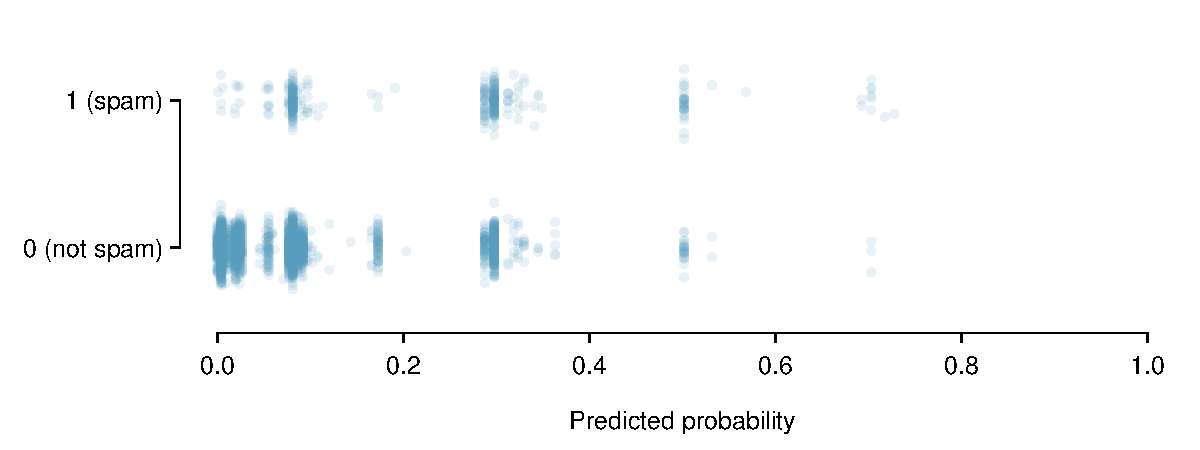
\includegraphics[width=\textwidth]{ch_regr_mult_and_log/figures/logisticModel/logisticModelPredict}
\caption{The predicted probability that each of the 3,912 emails is spam is classified by their grouping, spam or not. Noise (small, random vertical shifts) have been added to each point so that points with nearly identical values aren't plotted exactly on top of one another. This makes it possible to see more observations.}
\label{logisticModelPredict}
\end{figure}

This may at first seem very discouraging: we have fit a logistic model to create a spam filter, but no emails have a fitted probability of being spam above 0.75. Don't despair; we will discuss ways to improve the model through the use of better variables in Section~\ref{improvingTheSetOfVariablesForASpamFilter}.

We'd like to assess the quality of our model. For example, we might ask: if we look at emails that we modeled as having a 10\% chance of being spam, do we find about 10\% of them actually are spam? To help us out, we'll borrow an advanced statistical method called \term{natural splines} that estimates the local probability over the region 0.00 to 0.75 (the largest predicted probability was 0.73, so we avoid extrapolating). All you need to know about natural splines to understand what we are doing is that they are used to fit flexible lines rather than straight lines.

The curve fit using natural splines is shown in Figure~\ref{logisticModelSpline} as a solid black line. If the logistic model fits well, the curve should closely follow the dashed $y=x$ line. We have added shading to represent the confidence bound for the curved line to clarify what fluctuations might plausibly be due to chance. Even with this confidence bound, there are weaknesses in the first model assumption. The solid curve and its confidence bound dips below the dashed line from about 0.1 to 0.3, and then it drifts above the dashed line from about 0.35 to 0.55. These deviations indicate the model relating the parameter to the predictors does not closely resemble the true relationship.

\begin{figure}
\centering
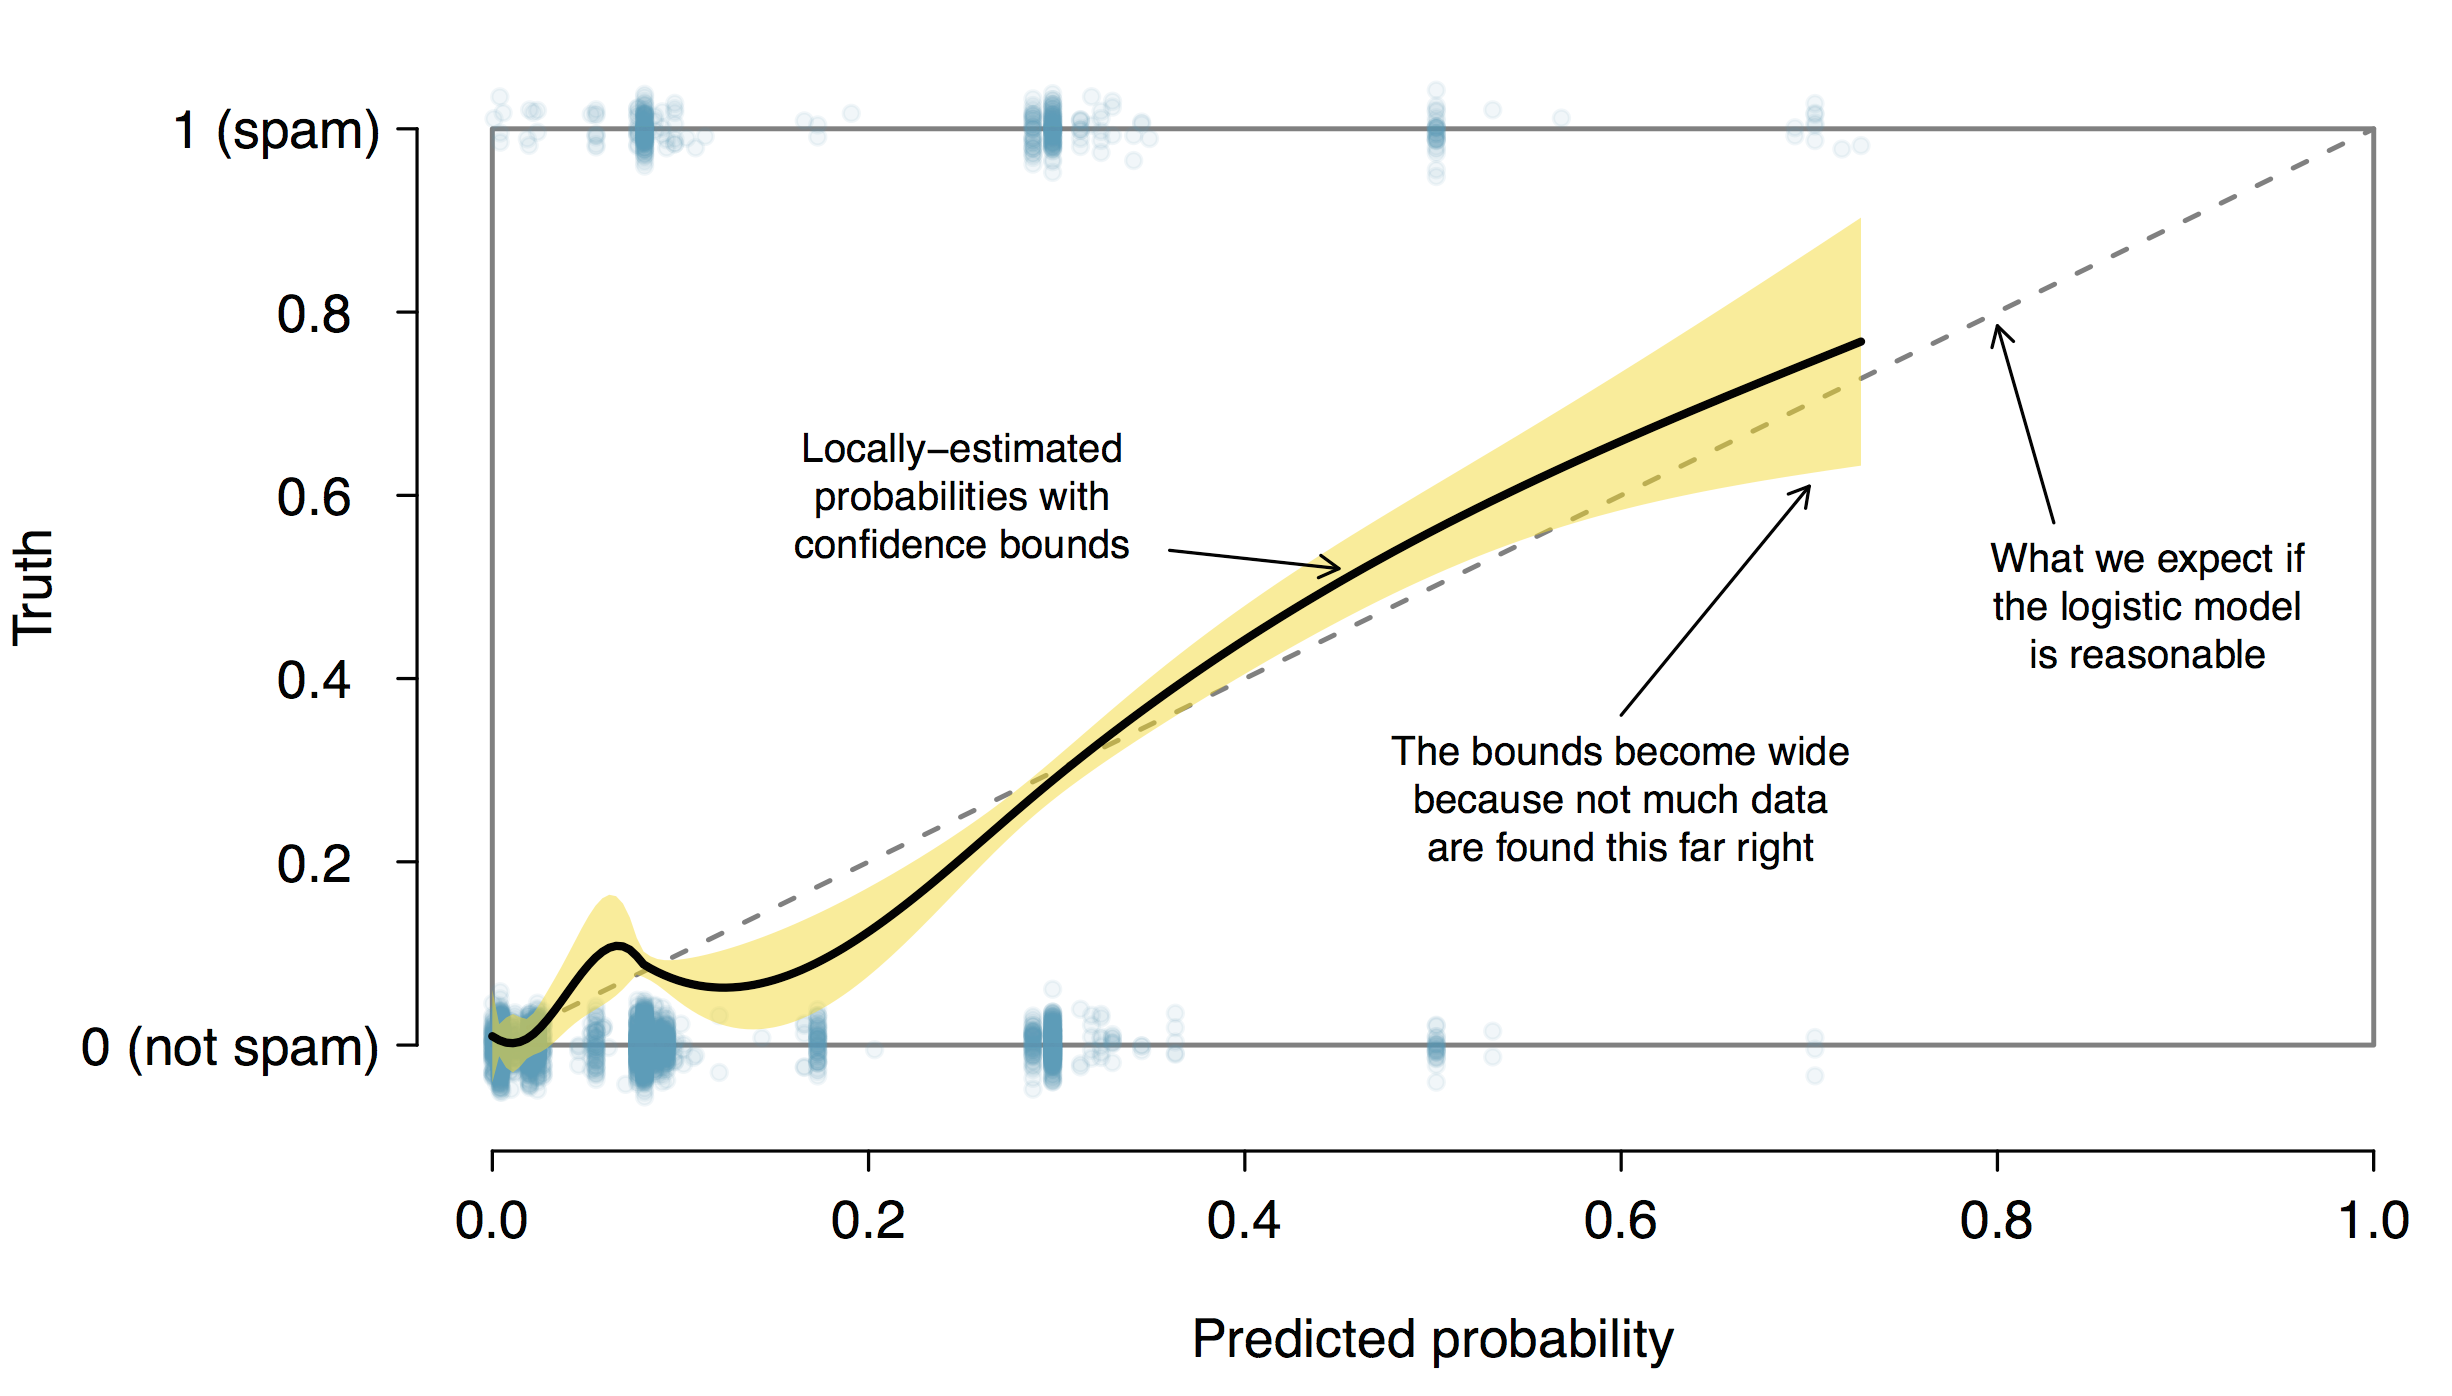
\includegraphics[width=\textwidth]{ch_regr_mult_and_log/figures/logisticModel/logisticModelSpline}
\caption{The solid black line provides the empirical estimate of the probability for observations based on their predicted probabilities (confidence bounds are also shown for this line), which is fit using natural splines. A small amount of noise was added to the observations in the plot to allow more observations to be seen.}
\label{logisticModelSpline}
\end{figure}

We could evaluate the second logistic regression model assumption -- independence of the outcomes -- using the model residuals. The residuals for a logistic regression model are calculated the same way as with multiple regression: the observed outcome minus the expected outcome. For logistic regression, the expected value of the outcome is the fitted probability for the observation, and the residual may be written as
\begin{align*}
e_i = Y_i - \hat{p}_i
\end{align*}
We could plot these residuals against a variety of variables or in their order of collection, as we did with the residuals in multiple regression. However, since the model will need to be revised to effectively classify spam and you have already seen similar residual plots in Section~\ref{multipleRegressionModelAssumptions}, we won't investigate the residuals here.


\textC{\pagebreak}


\subsection{Improving the set of variables for a spam filter}
\label{improvingTheSetOfVariablesForASpamFilter}

If we were building a spam filter for an email service that managed many accounts (e.g. Gmail or Hotmail), we would spend much more time thinking about additional variables that could be useful in classifying emails as spam or not. We also would use transformations or other techniques that would help us include strongly skewed numerical variables as predictors.

Take a few minutes to think about additional variables that might be useful in identifying spam. Below is a list of variables we think might be useful:
\begin{enumerate}
\item[(1)] An indicator variable could be used to represent whether there was prior two-way correspondence with a message's sender. For instance, if you sent a message to john@example.com and then John sent you an email, this variable would take value 1 for the email that John sent. If you had never sent John an email, then the variable would be set to~0.
\item[(2)] A second indicator variable could utilize an account's past spam flagging information. The variable could take value 1 if the sender of the message has previously sent messages flagged as~spam.
\item[(3)] A third indicator variable could flag emails that contain links included in previous spam messages. If such a link is found, then set the variable to~1 for the email. Otherwise, set it to~0.
\end{enumerate}
The variables described above take one of two approaches. Variable (1) is specially designed to capitalize on the fact that spam is rarely sent between individuals that have two-way communication. Variables~(2) and~(3) are specially designed to flag common spammers or spam messages. While we would have to verify using the data that each of the variables is effective, these seem like promising ideas.

Table~\ref{emailTableOfSpamAnd} shows a contingency table for spam and also for the new variable described in~(1) above. If we look at the 1,090 emails where there was correspondence with the sender in the preceding 30 days, not one of these message was spam. This suggests variable~(1) would be very effective at accurately classifying some messages as not spam. With this single variable, we would be able to send about 28\% of messages through to the inbox with confidence that almost none are spam.

\begin{table}[h]
\centering
\begin{tabular}{lrrrr}
& \multicolumn{3}{c}{prior correspondence} & \\
\cline{2-4}
 & \ \hspace{5mm}\resp{no} & \ \hspace{8mm}\resp{yes} && \ \hspace{3mm}Total \\
\hline
\vspace{-3.8mm} & & & & \\
\resp{spam} &  367 &    0 &&  367 \\
\resp{not spam}\hspace{3mm}\  & 2464 & 1090 && 3554 \\
\hline
\vspace{-3.8mm} & & & & \\
Total & 2831 & 1090 && 3921 \\
\hline
\end{tabular}
\caption{A contingency table for \var{spam} and a new variable that represents whether there had been correspondence with the sender in the preceding 30~days.}
\label{emailTableOfSpamAnd}
\end{table}
%library(openintro); data(email); contTable(email[,c("spam", "sent_email")])

The variables described in (2) and (3) would provide an excellent foundation for distinguishing messages coming from known spammers or messages that take a known form of spam. To utilize these variables, we would need to build databases: one holding email addresses of known spammers, and one holding URLs found in known spam messages. Our access to such information is limited, so we cannot implement these two variables in this textbook. However, if we were hired by an email service to build a spam filter, these would be important next steps.

In addition to finding more and better predictors, we would need to create a customized logistic regression model for each email account. This may sound like an intimidating task, but its complexity is not as daunting as it may at first seem. We'll save the details for a statistics course where computer programming plays a more central role.

For what is the extremely challenging task of classifying spam messages, we have made a lot of progress. We have seen that simple email variables, such as the format, inclusion of certain words, and other circumstantial characteristics, provide helpful information for spam classification. Many challenges remain, from better understanding logistic regression to carrying out the necessary computer programming, but completing such a task is very nearly within your reach.

\index{data!email|)}
\index{logistic regression|)}
